% ============================================================
%  article.tex — Yu-Gi-Oh! Card Interactions
%  Blibeche Farès — April 2026
% ============================================================
\documentclass[10pt, a4paper]{article}
\usepackage{config}

% ── Metadata ────────────────────────────────────────────────
\title{Are Yu-Gi-Oh!\ Cards Sharing the Same Type\\
       More Likely to Interact Together?}
\author{Blibeche Farès}
\journalheader{Are Yu-Gi-Oh!\ Cards Sharing the Same Type More Likely to Interact?}
\runningauthors{Blibeche, April 2026}
\studydate{April $2026$}

% ============================================================
\begin{document}
\thispagestyle{empty}
% ============================================================

\maketitle

\begin{paperabstract}
This study investigates whether pairs of Yu-Gi-Oh!\ cards sharing
the same monster type are more likely to interact together,
using a dataset of annotated card pairs produced by a
large language model (Llama $3.1$ $8$B). We fitted a multivariate regression
($R^2 = 0.02$) on monster-pairs, modelling the number of interactions between two cards
(\textit{interactCount}) as a function of shared type, shared
attribute, shared frametype, level difference, attack difference,
defence difference, and annotation-quality control features. Shared
type ($\beta = 0.18$, $p < 0.001$) and shared attribute
($\beta = 0.13$, $p < 0.001$) emerge as the strongest positive
predictors, while combat-stat differences show no significant
effect. Annotation-quality controls --- \textit{stability} ($\beta = -0.68$, $p < 0.001$) and
\textit{repeated} ($\beta = -0.34$, $p < 0.001$) --- carry large negative coefficients, 
indicating that the model's variability introduces noise that should be 
accounted for when interpreting the main effects.
\end{paperabstract}

\begin{keywords}
Yu-Gi-Oh!, card interactions, deck synergy, LLM annotation,
Llama $3.1$ $8$B, multivariate regression.
\end{keywords}

\startbody

% ============================================================
\section{Introduction}
% ============================================================

\lettrine[lines=4]{Y}{u-Gi-Oh!} is a Japanese trading card game in
which players assemble decks of $40-60$ cards and compete by summoning
monsters, activating spell and trap effects, and reducing the
opponent's life points to zero. With over $14{,}000$ unique cards in
circulation, understanding which cards work well together is one of
the most demanding cognitive tasks faced by competitive players.

Deck synergy --- the capacity of a set of cards to reinforce one
another through their effects --- is typically evaluated through
years of gameplay experience. In this study, we take a data-driven
approach to determine whether a simple structural feature of a card,
namely its \textbf{monster type} (Dragon, Warrior, Spellcaster,
etc.), is a statistically significant predictor of whether two cards
interact.

This question is motivated by the observation that the majority of
support cards in the game are formulated around the monster type. A
card that reads \textit{``Add $1$ Warrior monster from your Deck to
your hand''} explicitly targets cards sharing the Warrior type. If
this design principle is reflected in the data at scale, we would
expect same-type pairs to have significantly more interactions than
cross-type pairs.

\textbf{Question.} \textit{Are monster cards sharing the same type
significantly more likely to interact?}

\begin{figure}[H]
  \centering
  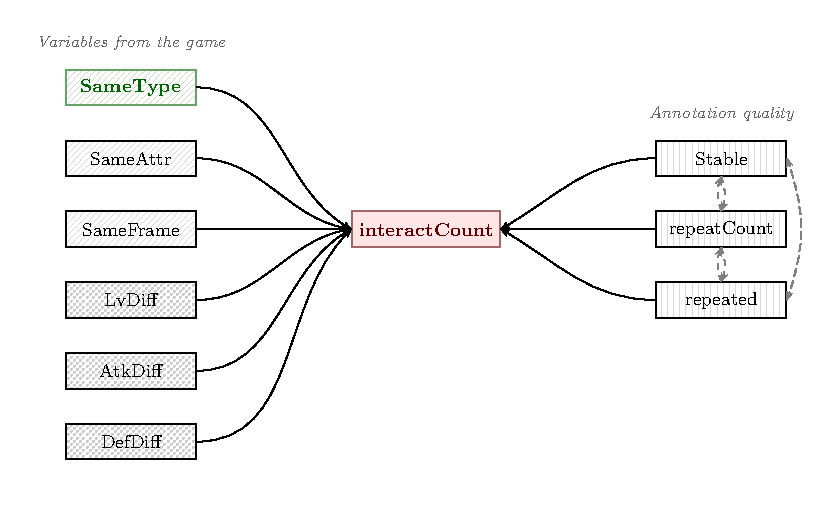
\includegraphics[width=1.03\linewidth, trim=5mm 2mm 5mm 2mm, clip]
    {DAG/directed_acyclic_graph.pdf}
  \caption{DAG representing our theory.}
  \label{fig:dag}
  \vspace{-12pt}
\end{figure}

% ============================================================
\section{Data}
% ============================================================

\subsection{Card Database}

Card data was extracted from the YGOProDeck API~\cite{ygoprodeck},
providing a dataset of $14{,}137$ cards~\cite{ygo_scrapping_data}.
Each card is described by its name, effect text, frametype (normal,
effect, fusion, synchro, xyz, link, spell, trap, etc.), monster type,
attribute (DARK, LIGHT, FIRE, WATER, WIND, EARTH), level, attack,
and defence. A full description of all variables is provided in
Table~\ref{tab:codebook}.

\subsection{Interaction Dataset}

A second dataset of $27{,}417$ directed card pairs
$(A \rightarrow B)$~\cite{ygo_interaction_data} was annotated by an
LLM (Llama $3.1$ $8$B) prompted with domain-specific instructions
(see Appendix~\ref{sec:prompt}). For each pair, the model produced a
binary label for each of $56$ interaction types
(e.g.\ \texttt{special\_summon}, \texttt{destroy}, \texttt{target},
\texttt{references\_type}). A subset of pairs was annotated multiple
times because of the probabilistic nature of sampling process (see Appendix~\ref{sec:quality}, 
Fig.~\ref{fig:stability}).

\widefig{Figures/distribution_interactions.png}{0.95}
  {Distribution of the number of active interactions per annotated
   row. The distribution is right-skewed: most pairs share zero or
   one interaction, while a small subset shares several.}
  {fig:dist}

% ============================================================
\section{Method}
% ============================================================

\subsection{Feature Engineering}

Starting from the raw interaction dataframe, we construct one
observation per unique directed pair. The response variable
\textit{interactCount} is the mean total number of active
interactions across all annotated occurrences of that pair:
\begin{equation}
  \textit{interactCount}_{p}
    = \frac{1}{|R_p|}\sum_{r \in R_p}\sum_{j=1}^{56} x_{rj}
  \label{eq:ic}
\end{equation}
where $R_p$ is the set of annotation rows for pair $p$ and $x_{r,j}$
is the binary label for interaction type $j$ in row $r$.

Two annotation-quality variables are computed. \textit{repeated} is
a binary indicator equal to $1$ if a pair was annotated more than
once. \textit{stability} equals $1$ if all repeated annotations
agree, $0$ otherwise.

Six card-level features are derived from card data:
\begin{itemize}
  \item \textbf{SameType} --- $1$ if cards $A$ and $B$ share the same
        monster type, else $0$.
  \item \textbf{SameAttr} --- $1$ if cards $A$ and $B$ share the same
        attribute, else $0$.
  \item \textbf{SameFrame} --- $1$ if cards $A$ and $B$ share the same
        frametype, else $0$.
  \item \textbf{LvDiff}, \textbf{AtkDiff}, \textbf{DefDiff} ---
        absolute differences in level, ATK, and DEF.
\end{itemize}

Pairs involving at least one spell or trap card are excluded,
retaining $9{,}518$ monster pairs. Continuous predictors are
standardised (mean~$0$, standard deviation~$1$). The causal
structure assumed by our model is represented by the DAG in
Fig.~\ref{fig:dag}.

\subsection{OLS Model}

We estimate the mean number of interactions per pair as a linear
function of the nine predictors described above:
\begin{equation}
  \textit{interactCount}_i
    = \beta_0 + \sum_{k=1}^{9}\beta_k\,x_{k,i} + \varepsilon_i
  \label{eq:ols}
\end{equation}
where $x_{1..9}$ are, in order, \textit{SameType}, \textit{SameAttr},
\textit{SameFrame}, \textit{LvDiff}, \textit{AtkDiff},
\textit{DefDiff}, \textit{stability}, \textit{repeatCount}, and
\textit{repeated}. The model is estimated using \texttt{statsmodels}
(Python~$3$). Coefficients, confidence intervals, and
$p$-values are reported and visualised as a forest plot.

% ============================================================
\section{Results}
% ============================================================

\widefig{Figures/forest_plot.png}{0.90}
  {Forest plot of OLS coefficients with confidence intervals.
   Red points: $p < 0.05$. Grey points: non-significant.
   Red dashed line: zero effect.}
  {fig:forest}

\subsection{Descriptive Statistics}

Fig.~\ref{fig:dist} shows the distribution of \textit{interactCount}
across all annotated rows: right-skewed, with the majority of pairs
sharing zero or one interaction. Fig.~\ref{fig:features} shows the
distribution of binary predictors in the monster-pair subset:
same-type pairs are the least frequent ($13.0\%$), while
same-attribute ($24.8\%$) and same-frametype ($52.2\%$) pairs are
more common.

\subsection{Regression Results}

Table~\ref{tab:coefs} summarises the estimated coefficients
($n = 9{,}518$, $R^2 = 0.024$). The forest plot in
Fig.~\ref{fig:forest} visualises the confidence intervals
for each predictor.

\resulttable
  {OLS estimates. Significant predictors ($p < 0.05$) are bolded.}
  {tab:coefs}
  {
    \textbf{Intercept}    & $\mathbf{1.179}$  & $\mathbf{<0.001}$ \\
    \textbf{SameType}     & $\mathbf{0.178}$  & $\mathbf{<0.001}$ \\
    \textbf{SameAttr}     & $\mathbf{0.133}$  & $\mathbf{<0.001}$ \\
    \textbf{SameFrame}    & $\mathbf{-0.036}$ & $\mathbf{0.026}$  \\
    LvDiff                & $0.008$           & $0.413$           \\
    AtkDiff               & $0.000$           & $0.974$           \\
    DefDiff               & $0.008$           & $0.366$           \\
    \textbf{stability}    & $\mathbf{-0.682}$ & $\mathbf{<0.001}$ \\
    \textbf{repeatCount}  & $\mathbf{-0.023}$ & $\mathbf{0.027}$  \\
    \textbf{repeated}     & $\mathbf{-0.337}$ & $\mathbf{<0.001}$ \\
  }

\subsection{Interpretation}

\textbf{SameType} is the strongest positive predictor: same-type
pairs have on average $0.18$ more interactions than cross-type
pairs, after controlling for all other variables. \textbf{SameAttr}
shows a comparable positive effect. \textbf{SameFrame} carries a
small but significant \emph{negative} coefficient, reflecting the
fact that pairs drawn from the same frametype (e.g.\ two normal
monsters) often interact through external support cards rather than
directly. Combat-stat differences (\textit{LvDiff}, \textit{AtkDiff},
\textit{DefDiff}) are all non-significant. The large negative
coefficients on \textit{stability} and \textit{repeated} indicate
that repeated annotations tend to converge towards lower interaction
counts, reflecting LLM variability in borderline cases; this
motivates including these controls rather than ignoring them.

% ============================================================
\section{Discussion \& Limitations}
% ============================================================

Our results are consistent with the design philosophy of Yu-Gi-Oh!.
The game's support cards are systematically formulated around
monster types, which naturally creates type-homogeneous interaction
clusters.

Several limitations apply. The dataset covers only a fraction of the
complete pairwise space ($27{,}417$ annotations out of more than
$10^{8}$ possible pairs), and its representativeness cannot be
guaranteed. The assumption that LLM annotations approximate
human-quality labels cannot be formally verified without
gold-standard human annotations (that I am working on, through a collaborative annotation website project); 
the significance of the annotation-quality controls indicates real noise in the labelling
process. Finally, the model explains only a modest fraction of
variance in \textit{interactCount} ($R^2 = 0.02$), indicating that
card-effect text --- not captured in our feature set --- accounts
for most of the remaining variation.

% ============================================================
\section{Conclusion}
% ============================================================

This study demonstrates that \textbf{shared monster type is a
significant positive predictor of card interaction count} in
Yu-Gi-Oh!, after controlling for shared attribute, shared frametype,
combat-stat differences, and LLM annotation quality. The result is
directly interpretable for a player: building a deck around a single
monster type maximises the probability that your cards interact with
one another.

Future work could incorporate archetype (that is very difficult to define here), 
a rule-based relevant pairs selector (such as "in conditions" used in this last study~\cite{ygo_individualism})
to extract more cases of interactions and start use interaction types,
or use graph-based methods to identify the most central cards within
type-specific interaction networks. Graph-based analytics seems to be very promising in understanding underlying structures
of the game, and quantify deck synergy.

\finalornament

\stopbody

% ── Bibliography ─────────────────────────────────────────────
\begingroup
\small
\bibliography{references}
\endgroup

% ============================================================
\begin{appendices}

% ── A. Variable Codebook ─────────────────────────────────────
\section{Variable Codebook}
\label{sec:codebook}

\apptable
  {Description of all variables used in the analysis.}
  {tab:codebook}
  {llp{7cm}l}
  {
    \textbf{Source} & \textbf{Variable} & \textbf{Description} & \textbf{Type} \\
    \midrule
    \multirow{6}{*}{Cards API}
      & \texttt{type}      & Monster type (Dragon, Warrior, \ldots)          & Categorical \\
      & \texttt{attribute} & Attribute (DARK, LIGHT, FIRE, \ldots)           & Categorical \\
      & \texttt{frametype} & Frametype (effect, fusion, \ldots)              & Categorical \\
      & \texttt{level}     & Monster level ($0$--$12$)                       & Integer     \\
      & \texttt{atk}       & ATK value ($0$--$5000$)                         & Integer     \\
      & \texttt{defe}      & DEF value ($0$--$5000$)                         & Integer     \\
    \midrule
    \multirow{3}{*}{Shared Features}
      & \texttt{sharedType}      & $1$ if both cards share monster type      & Binary \\
      & \texttt{sharedAttribute} & $1$ if both cards share attribute         & Binary \\
      & \texttt{sharedFrametype} & $1$ if both cards share frametype         & Binary \\
    \midrule
    \multirow{3}{*}{Stat diff.}
      & \texttt{lvDiff}  & $|\text{level}_A - \text{level}_B|$, standardised & Continuous \\
      & \texttt{atkDiff} & $|\text{ATK}_A - \text{ATK}_B|$, standardised     & Continuous \\
      & \texttt{defDiff} & $|\text{DEF}_A - \text{DEF}_B|$, standardised     & Continuous \\
    \midrule
    \multirow{4}{*}{Annotation}
      & \texttt{interactCount} & Mean total interactions per pair            & Continuous \\
      & \texttt{repeatCount}   & Number of annotations of pair, standardised & Continuous \\
      & \texttt{repeated}      & $1$ if pair was annotated more than once    & Binary     \\
      & \texttt{stability}     & $1$ if all pair annotations agree           & Binary     \\
  }

% ── B. Annotation Quality ────────────────────────────────────
\section{Annotation Quality Diagnostics}
\label{sec:quality}

\begin{figure}[H]
  \centering
  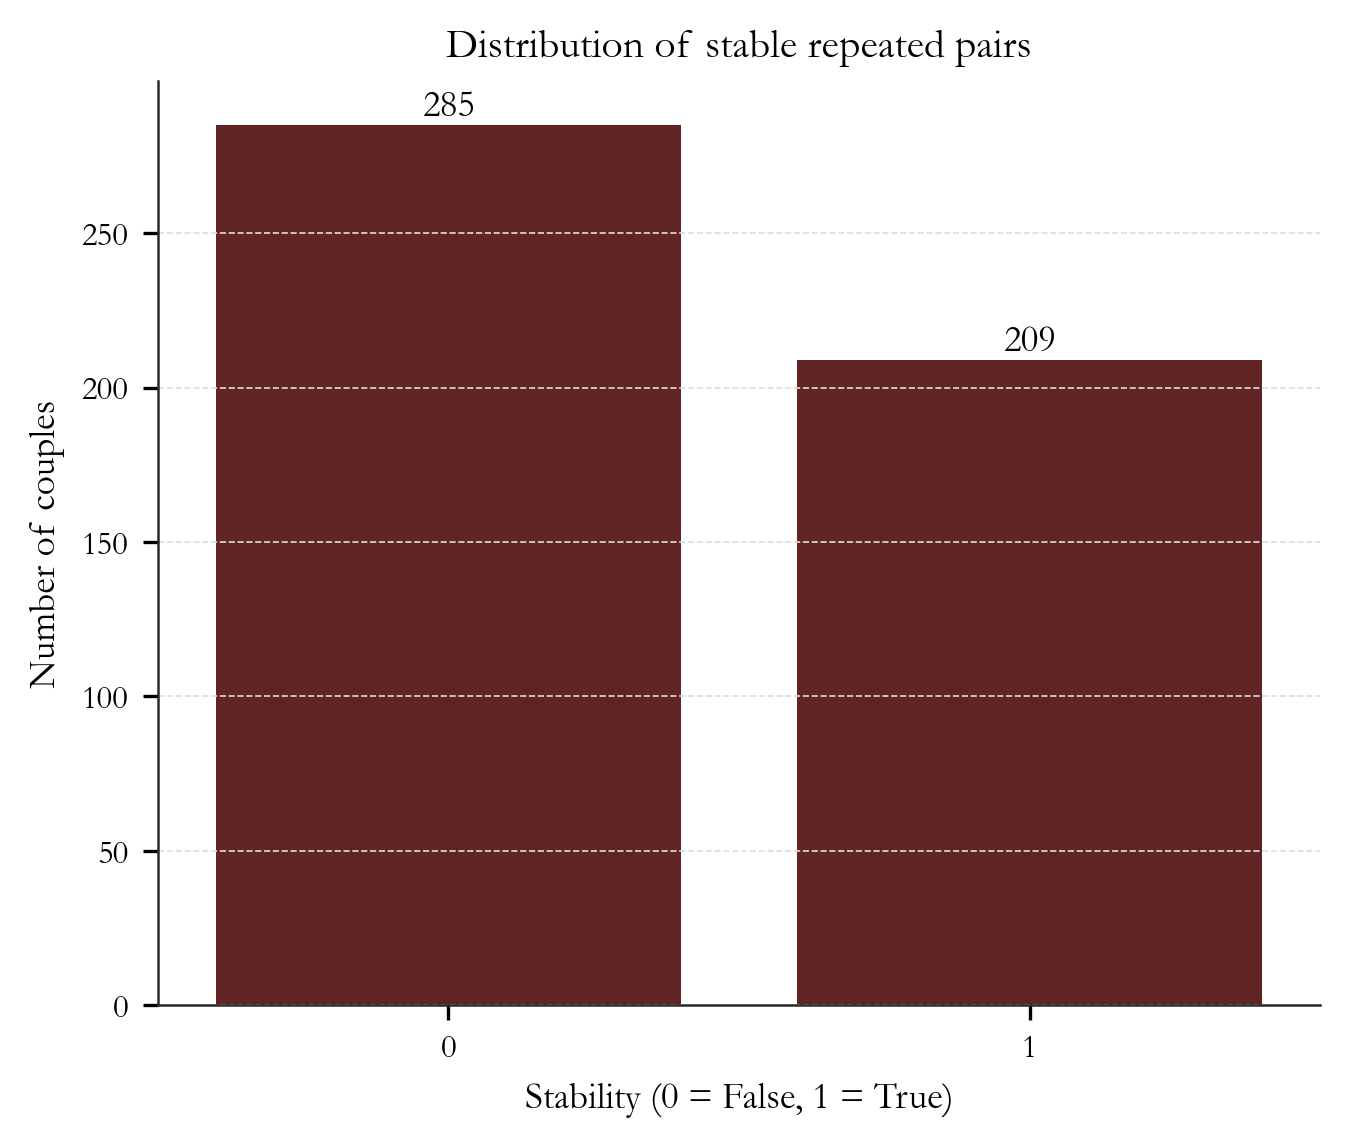
\includegraphics[width=0.72\textwidth]{Figures/distribution_stability.png}
  \caption{Distribution of \textit{stability} among repeated pairs
    ($0$: inconsistent, $1$: consistent).}
  \label{fig:stability}
\end{figure}

\begin{figure}[H]
  \centering
  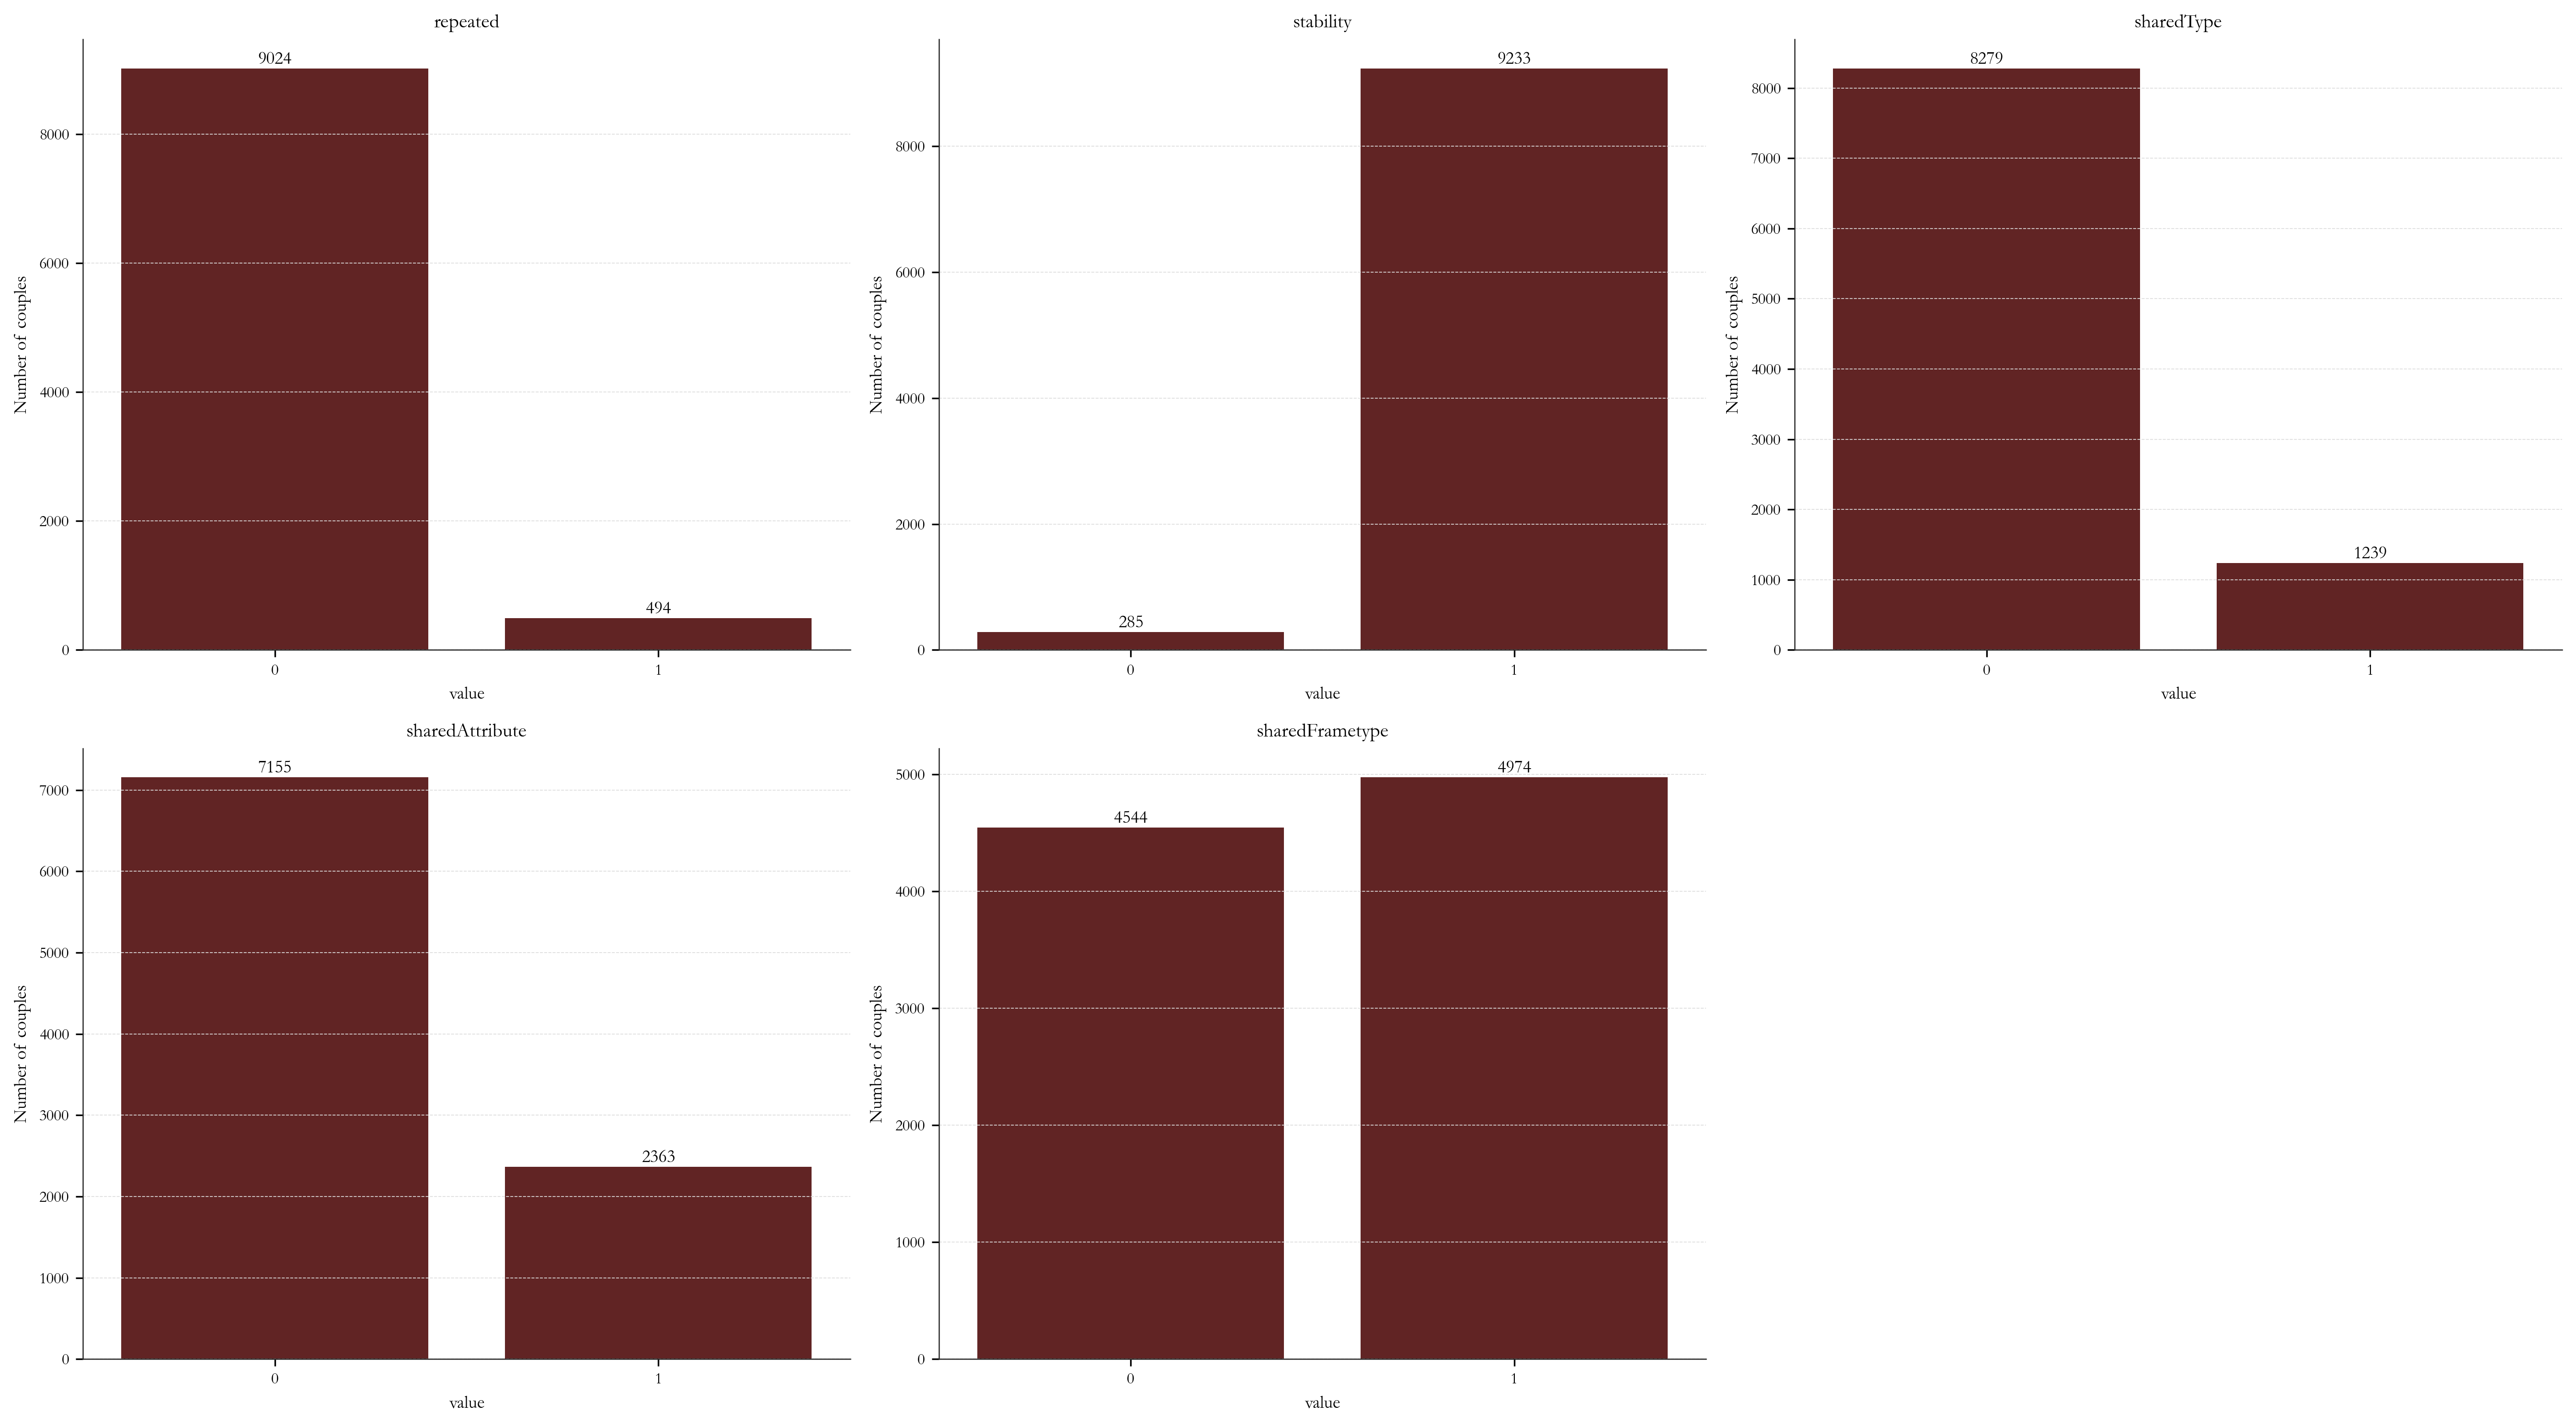
\includegraphics[width=0.95\textwidth]{Figures/features_binary_values.png}
  \caption{Distributions of binary features (\textit{SameType},
    \textit{SameAttr}, \textit{SameFrame}) in the monster-pair
    subset used for regression.}
  \label{fig:features}
\end{figure}

% ── C. LLM Prompt Summary ────────────────────────────────────
\section{LLM Annotation Prompt Summary}
\label{sec:prompt}

The LLM (Llama $3.1$ $8$B) was prompted to identify directed
interactions from Card~$A$ to Card~$B$ only, under the
assumption that both cards are used from the same player. The model was provided with:
\begin{sloppypar}
\begin{itemize}
  \item The full effect text and data (type, attribute,
        frametype, level, ATK, DEF) of both cards.
  \item A glossary of $56$ allowed relation types
        (e.g.\ \texttt{special\_summon}, \texttt{destroy},
        \texttt{references\_type}, \texttt{buff\_atk},
        \texttt{negate\_effect}).
  \item $13$ annotated examples covering edge cases such as
        opponent-only effects and generic mass effects.
\end{itemize}
\end{sloppypar}
The model returned a JSON object listing applicable relation types
with supporting evidence text and a confidence score. The full
procedure is documented in \texttt{automated\_annotator.ipynb}.


% ── D. Per-Variable Interaction Distributions ────────────────
\section{Per-Variable Interaction Distributions}
\label{sec:interactions}

\vspace{6pt}

% Helper : inline miniplot, no subfigure/caption wrapper
\newcommand{\miniplot}[1]{%
  \includegraphics[width=0.235\textwidth]%
    {Figures/interactions_variables/#1.png}%
}

\noindent
\miniplot{mentions_name}\hfill
\miniplot{mentions_archetype}\hfill
\miniplot{references_type}\hfill
\miniplot{references_attribute}\\[2pt]
\miniplot{references_level}\hfill
\miniplot{references_atk}\hfill
\miniplot{references_def}\hfill
\miniplot{references_frametype}\\[2pt]
\miniplot{references_archetype}\hfill
\miniplot{normal_summon}\hfill
\miniplot{special_summon}\hfill
\miniplot{tribute_summon}\\[2pt]
\miniplot{fusion_summon}\hfill
\miniplot{synchro_summon}\hfill
\miniplot{xyz_summon}\hfill
\miniplot{link_summon}\\[2pt]
\miniplot{pendulum_summon}\hfill
\miniplot{search_deck}\hfill
\miniplot{add_to_hand}\hfill
\miniplot{set_from_deck}\\[2pt]
\miniplot{mill_from_deck}\hfill
\miniplot{excavate_deck}\hfill
\miniplot{send_to_graveyard}\hfill
\miniplot{revive_from_graveyard}\\[2pt]
\miniplot{banish}\hfill
\miniplot{return_from_graveyard}\hfill
\miniplot{return_to_hand}\hfill
\miniplot{return_to_deck}\\[2pt]
\miniplot{destroy}\hfill
\miniplot{target}\hfill
\miniplot{equip}\hfill
\miniplot{unequip}\\[2pt]
\miniplot{buff_atk}\hfill
\miniplot{buff_def}\hfill
\miniplot{reduce_atk}\hfill
\miniplot{reduce_def}\\[2pt]
\miniplot{change_level}\hfill
\miniplot{change_attribute}\hfill
\miniplot{change_type}\hfill
\miniplot{protect_monster}\\[2pt]
\miniplot{protect_effects}\hfill
\miniplot{negate_activation}\hfill
\miniplot{negate_effect}\hfill
\miniplot{cannot_be_destroyed}\\[2pt]
\miniplot{cannot_be_targeted}\hfill
\miniplot{take_control}\hfill
\miniplot{change_control}\hfill
\miniplot{cannot_attack}\\[2pt]
\miniplot{force_attack}\hfill
\miniplot{direct_attack}\hfill
\miniplot{piercing_damage}\hfill
\miniplot{draw_cards}\\[2pt]
\miniplot{discard}\hfill
\miniplot{pay_lp}\hfill
\miniplot{gain_lp}\hfill
\miniplot{skip_phase}\\[4pt]

\captionof{figure}{Distribution of each of the $56$ interaction
  types across the $27{,}417$ annotated pairs. For each subplot,
  the left bar counts $x = 0$ (interaction absent), the right bar
  counts $x = 1$ (interaction present).}
\label{fig:interactions_all}


\end{appendices}

\end{document}